\documentclass[12pt,letterpaper, onecolumn]{exam}
\usepackage{amsmath}
\usepackage{amssymb}
\usepackage{sidecap}
\usepackage{tabularx}
\usepackage{csquotes}
\usepackage{makecell}
\usepackage{hyperref}
\hypersetup{
    colorlinks=true,
    linkcolor=blue,
    filecolor=magenta,      
    urlcolor=black,
    pdftitle={Overleaf Example},
    pdfpagemode=FullScreen,
}
%\usepackage[left=0.5cm,right=0.5cm,top=0.5cm,bottom=0.5cm]{geometry}
\usepackage[usestackEOL]{stackengine}
%\setstacktabbedgap{1ex} 
\usepackage{tikz}
\usetikzlibrary{decorations.pathreplacing}
\usetikzlibrary{fadings}
\def\layersep{2.5cm}

\usepackage{enumitem}

%\usepackage[shortlabels]{enumitem}
%\usepackage{enumerate}
\usepackage[lmargin=71pt, tmargin=0.8in]{geometry}  %For centering solution box

% \chead{\hline} % Un-comment to draw line below header
\thispagestyle{empty}   %For removing header/footer from page 1
\usepackage{color}
\definecolor{light-gray}{gray}{0.95}

\usepackage{listings}
\lstset{
    basicstyle=\footnotesize\ttfamily,
    escapechar=¢,
    language=python,
    frame=single,
    frameround=tttt,
    showstringspaces=false,
    backgroundcolor=\color{light-gray}
}
\newcommand*{\ipythonprompt}[1]{\makebox[0pt][r]{\textbf{In [#1]:}\hspace{1em}}}

\usepackage{xcolor}

\definecolor{codegreen}{rgb}{0,0.6,0}
\definecolor{codegray}{rgb}{0.5,0.5,0.5}
\definecolor{codepurple}{rgb}{0.58,0,0.82}
\definecolor{backcolour}{rgb}{0.95,0.95,0.92}

\lstdefinestyle{mystyle}{
    backgroundcolor=\color{light-gray},   
    commentstyle=\color{codegreen},
    keywordstyle=\color{magenta},
    numberstyle=\tiny\color{codegray},
    stringstyle=\color{codepurple},
    basicstyle=\ttfamily\footnotesize,
    breakatwhitespace=false,         
    breaklines=true,                 
    captionpos=b,                    
    keepspaces=true,                 
    numbers=left,                    
    numbersep=5pt,                  
    showspaces=false,                
    showstringspaces=false,
    showtabs=false,                  
    tabsize=2
}

\lstset{style=mystyle}




\begin{document}



\newtheorem{theorem}{Theorem}[section]
\newtheorem{problem}{Problem}
\newtheorem{proposition}{Proposition}[section]
\newtheorem{lemma}{Lemma}[section]
\newtheorem{corollary}[theorem]{Corollary}
\newtheorem{example}{Example}[section]
\newtheorem{definition}[problem]{Definition}

\newcommand{\BEQA}{\begin{eqnarray}}
\newcommand{\EEQA}{\end{eqnarray}}
\newcommand{\define}{\stackrel{\triangle}{=}}
\bibliographystyle{IEEEtran}
\raggedbottom
\setlength{\parindent}{0pt}
\providecommand{\mbf}{\mathbf}
\providecommand{\norm}[1]{\lVert#1\rVert}
\providecommand{\pr}[1]{\ensuremath{\Pr\left(#1\right)}}
\providecommand{\qfunc}[1]{\ensuremath{Q\left(#1\right)}}
\providecommand{\sbrak}[1]{\ensuremath{{}\left[#1\right]}}
\providecommand{\lsbrak}[1]{\ensuremath{{}\left[#1\right.}}
\providecommand{\rsbrak}[1]{\ensuremath{{}\left.#1\right]}}
\providecommand{\brak}[1]{\ensuremath{\left(#1\right)}}
\providecommand{\lbrak}[1]{\ensuremath{\left(#1\right.}}
\providecommand{\rbrak}[1]{\ensuremath{\left.#1\right)}}
\providecommand{\cbrak}[1]{\ensuremath{\left\{#1\right\}}}
\providecommand{\lcbrak}[1]{\ensuremath{\left\{#1\right.}}
\providecommand{\rcbrak}[1]{\ensuremath{\left.#1\right\}}}
\let\vec\mathbf

\newlist{mydesc}{description}{1} % create a new list called mydesc, of type "description"
\setlist[mydesc]{
  align=left, % use the align-format defined above
  leftmargin=0pt, % indentation for all the lines
  labelindent=1em, % horizontal space before label
  labelsep=0pt
   % horizontal space after label -- set to zero because we add space via "leftwithbar"
}



\begingroup  
    \centering
    
    \LARGE Weekly Report 2 - K-Means\\[0.5em]
    
    \large Ganji Varshitha\par
    \large AI20BTECH11009\par
\endgroup
\rule{\textwidth}{0.4pt}
\pointsdroppedatright   %Self-explanatory
\printanswers
\newcommand\Solution{
  \textbf{Solution:}\\}
\newcommand{\myvec}[1]{\ensuremath{\begin{bmatrix}#1\end{bmatrix}}}
 %Replace "Ans:" with starting keyword in solution box

 \subsection*{Introduction}
K-Means is an unsupervised learning algorithm which performs partitioned clustering. Clustering helps us to understand the structure of the data by grouping it into distinct sub-groups.
\subsection*{Algorithm}

It is a parametric method where we need to specify the number of clusters K, which we want to divide the data into.
\\It is a simple and iterative algorithm described as follows:
\begin{mydesc}
 \item[\hspace{2cm}]\textmd{Initialize K random points from the dataset as centroids}
  \item[\hspace{2cm}]\textmd{\textbf{repeat}}
  \item[\hspace{3cm}]\textmd{Form K clusters by assigning all points to the closest centroid}
  \item[\hspace{3cm}]\textmd{Recompute the centroid of each cluster}
  \item[\hspace{2cm}]\textmd{\textbf{until} The centroids don't change}
 \end{mydesc}

It can be seen as Expectation-Maximisation problem where the E-step is assigning the data points to the closest cluster and the M-step is computing the centroid of each cluster.\\
It minimises the intra-cluster sum of squared distance from its centroid and keeps the clusters distant from each other.

\subsection*{Evaluation metric}
\textbf{SSE - Elbow method}\\
Since it is an unsupervised learning model, we don't have ground truth values to evaluate its performance. Hence, we select the model with a K value which minimises sum of squared distances between data points and its centroids.\\
When SSE is plotted against K, select the K where the graph flatten out and forms an elbow. This method is referred to as elbow method.
\newpage
\begin{figure}[!h]
\caption{Elbow method plot example}
\centering
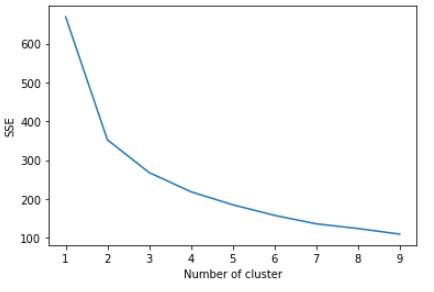
\includegraphics[width = 0.4\textwidth]{../images/elbowmethod.png}
\end{figure}

\subsection*{Code Example}
Generated data using gaussian distribution and took user defined values for K and input dimensions.

\subsubsection*{Data generation}
\begin{lstlisting}
¢\ipythonprompt{1}¢ 
NUM_PTS=3
#Accepting input dimensions(p) and number of clusters(k)
Y=np.empty((p,k*NUM_PTS),int)
p=int(input("Enter input dimensions: "))
k=int(input("Enter number of clusters:"))
#contains the data points of all the clusters
#declaring positive semi definite covariance matrix
cov=[]
y=[]

#Generating clusters using Gaussian distribution
for i in range(k):
  #declaring mean matrix
  mean=np.random.randint(i+1,p+i+1,p,int)
  cov=np.diag([i for j in range(p)])
  y=np.random.multivariate_normal(mean,cov,NUM_PTS).T
  Y=np.concatenate((Y,y),axis=1)
\end{lstlisting} 

\subsubsection*{Declaring stopping condition and implementing the algorithm}

\begin{lstlisting} 
¢\ipythonprompt{2}¢   
#Setting stopping condition
#epsilon = 0.001
# Initialize error to a large value
#error = 10000.0
# Initialize centroids - assume 4 of them from a 2D Gaussian distribution (zero mean, unit variance)
D = np.random.multivariate_normal(np.zeros(p), np.identity(p), k).T 
# Initialize iteration count to 0
count = 0
# Initialize cluster size to 0
num=np.zeros(k)
# Initialize centroid update to 0
centr= np.zeros((p, k))

#Initialise distance_vector
distance_vector=[]


while (error > epsilon):
  
  # Update clusters based on distance
  for idx in range(k*NUM_PTS):
    cur_y = Y[:,idx]
    print(cur_y)
    for j in range(k):
      cur_d=D[:,j]
      d1=np.sqrt(np.sum((cur_y-cur_d)**2))
      distance_vector.append(d1)
    # Find closest centroid 
    min_idx = distance_vector.index(np.min(distance_vector))
    for i in range(k):
      if (min_idx==i):
        num[i]+=1
        for j in range(p):
          centr[j,i]+=cur_y[j]
          if (num[i]!=0):
            centr[j,i]=centr[j,i]/num[i]
  
  error=np.sqrt(np.sum((centr-D)**2))
  for i in range(k):
    for j in range(p):
      D[j,i]=centr[j,i] 
  count+=1 
\end{lstlisting}



\subsection*{ Key points}
\begin{itemize}
\item The algorithm clusters the data into distinct sub groups which will not work for overlapping clusters.
\item Normalization is required as it deals with distances.
\item It assumes spherical shapes of clusters with center as  centroid and fails in case of complex designs or even elliptical shape.
\item The algorithm works well with large datasets and easy to implement.
\item The centroids are sensitive to outliers.
\item The algorithm is stochastic as the clusters formed depend on centroid initialisation.
\end{itemize}

\subsection*{Questions}
\begin{questions}
\question[] Does the cost function of the algorithm has an optimized solution?
\begin{Solution}
Objective function is given by
\begin{align*}
\arg \min \sum_{i=1}^K \sum_{x\in S_i} ||x - C_i||^2
\end{align*}
This function is a NP hard problem. Therefore, we only use Lloyd algorithm to stop iterating if the problem converges.\\
Since most of the convergence takes place in first few iterations, stopping condition is changed to $'$Until relatively few points change clusters$'$.
\end{Solution}
\question[] Illustrate an example where K means fails when clusters have complex design.\\
\begin{Solution}
\begin{figure}[!h]
\caption{K means for non spherical clusters}
\centering
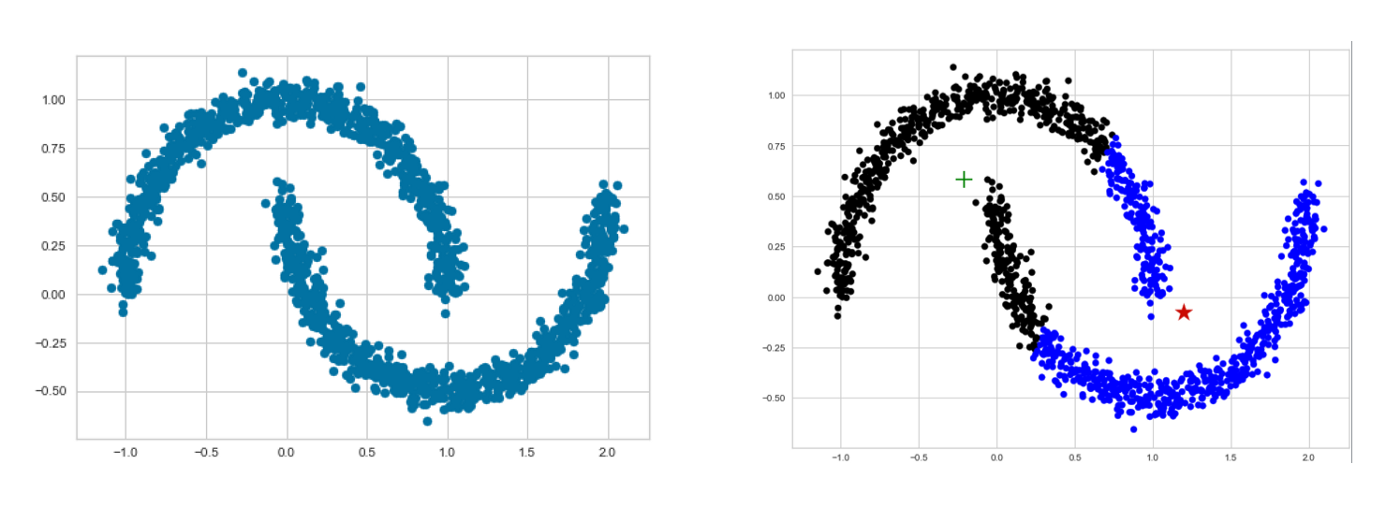
\includegraphics[width = 0.6\textwidth]{../images/k means.png}
\end{figure}

\end{Solution}
\end{questions}






\end{document}